%%%%%%%%%%%%%%%%%%%%%%%%%%%%%%%%%%%%%%%%%%%%%%%%%%%%%%%%%%%%
%%  Class 34, NE 155
%%

\documentclass[xcolor=x11names,compress]{beamer}

\definecolor{CoolBlack}{rgb}{0.0, 0.18, 0.39}
%% General document %%%%%%%%%%%%%%%%%%%%%%%%%%%%%%%%%%
\usepackage{graphicx}
\usepackage{tikz}
\usetikzlibrary{decorations.fractals}
\usepackage{hyperref}
%%%%%%%%%%%%%%%%%%%%%%%%%%%%%%%%%%%%%%%%%%%%%%%%%%%%%%

%% Beamer Layout %%%%%%%%%%%%%%%%%%%%%%%%%%%%%%%%%%
\useoutertheme[subsection=false,shadow]{miniframes}
\useinnertheme{default}
\usefonttheme{serif}
\usepackage{palatino}
\usepackage{tabu}
% Links
\usepackage{hyperref}
\definecolor{links}{HTML}{003262}
\hypersetup{colorlinks,linkcolor=,urlcolor=links}

% addition of color
\usepackage{xcolor}
\definecolor{CoolBlack}{rgb}{0.0, 0.18, 0.39}
\definecolor{byellow}{rgb}{0.55037, 0.38821, 0.06142}
\definecolor{dgreen}{rgb}{0.,0.6,0.}
\definecolor{RawSienna}{cmyk}{0,0.72,1,0.45}
\definecolor{forestgreen(web)}{rgb}{0.13, 0.55, 0.13}
\definecolor{cardinal}{rgb}{0.77, 0.12, 0.23}

\setbeamerfont{title like}{shape=\scshape}
\setbeamerfont{frametitle}{shape=\scshape}

\setbeamercolor*{lower separation line head}{bg=CoolBlack}
\setbeamercolor*{normal text}{fg=black,bg=white}
\setbeamercolor*{alerted text}{fg=dgreen} % just testing; I think this looks better
\setbeamercolor*{example text}{fg=black}
\setbeamercolor*{structure}{fg=black}

\setbeamercolor*{palette tertiary}{fg=black,bg=black!10}
\setbeamercolor*{palette quaternary}{fg=black,bg=black!10}

% Margins
\usepackage{changepage}

\mode<presentation>
{
  \definecolor{berkeleyblue}{HTML}{003262}
  \definecolor{berkeleygold}{HTML}{FDB515}
  \usetheme{Boadilla}      % or try Darmstadt, Madrid, Warsaw, Boadilla...
  %\usecolortheme{dove} % or try albatross, beaver, crane, ...
  \setbeamercolor{structure}{fg=berkeleyblue,bg=berkeleygold}
  \setbeamercolor{palette primary}{bg=berkeleyblue,fg=white} % changed this
  \setbeamercolor{palette secondary}{fg=berkeleyblue,bg=berkeleygold} % changed this
  \setbeamercolor{palette tertiary}{bg=berkeleyblue,fg=white} % changed this
  \usefonttheme{structurebold}  % or try serif, structurebold, ...
  \useinnertheme{circles}
  \setbeamertemplate{navigation symbols}{}
  \setbeamertemplate{caption}[numbered]
  \usebackgroundtemplate{}
}
%---

\renewcommand{\(}{\begin{columns}}
\renewcommand{\)}{\end{columns}}
\newcommand{\<}[1]{\begin{column}{#1}}
\renewcommand{\>}{\end{column}}

% adding slide numbers
\addtobeamertemplate{navigation symbols}{}{%
    \usebeamerfont{footline}%
    \usebeamercolor[fg]{footline}%
    \hspace{1em}%
    \insertframenumber/\inserttotalframenumber
}

% equation stuff
\newcommand{\Macro}{\ensuremath{\Sigma}}
\newcommand{\Sn}{\ensuremath{S_N} }
\newcommand{\vOmega}{\ensuremath{\hat{\Omega}}}
\usepackage{mathrsfs}
\usepackage[mathcal]{euscript}
\usepackage{amssymb}
\usepackage{amsthm}
\usepackage{epsfig}
\usepackage{amsmath}
%%%%%%%%%%%%%%%%%%%%%%%%%%%%%%%%%%%%%%%%%%%%%%%%%%
% title stuff for footer
\title{NE 155}
\author{R.\ N.\ Slaybaugh \\
(well, Max Fratoni!)}
\date{April 17, 2015}

\begin{document}

%%%%%%%%%%%%%%%%%%%%%%%%%%%%%%%%%%%%%%%%%%%%%%%%%%%%%%
%%%%%%%%%%%%%%%%%%%%%%%%%%%%%%%%%%%%%%%%%%%%%%%%%%%%%%
\begin{frame}
\title{NE 155\\Introduction to Numerical Simulations in Radiation Transport}
\subtitle{Lecture 34: Random Sampling}
\titlepage
\end{frame}


%%%%%%%%%%%%%%%%%%%%%%%%%%%%%%%%%%%%%%%%%%%%%%%%%%%%%%
%%%%%%%%%%%%%%%%%%%%%%%%%%%%%%%%%%%%%%%%%%%%%%%%%%%%%%
\begin{frame}{Major Components of MC Algorithm}

\begin{itemize}
  \item \textit{\textbf{PDFs}: the physical/mathematical system must be described by a set of pdfs.}
  % This class
  \item \textbf{Random number generator}: a source of random \#s uniformly distributed on the unit interval.
  % We're going to skip this
  \item \textit{\textbf{Sampling rule}: prescription for sampling the pdf (given having random \#s)}
  % This class
  \item \textbf{Scoring}: the outcomes must be accumulated/\underline{tallied} for quantities of interest
  % we might cover it
  \item \textbf{Error estimation}: an estimate of the statistical error (\underline{variance}) of the solution
  % Last class
  \item \textbf{Variance Reduction}: methods for reducing the variance and computation time simultaneously
  % briefly last class, maybe more at the end
  \item \textbf{Parallelization}: efficient use of computers
  % probably not
\end{itemize}
\end{frame}


%%%%%%%%%%%%%%%%%%%%%%%%%%%%%%%%%%%%%%%%%%%%%%%%%%%%%%
%%%%%%%%%%%%%%%%%%%%%%%%%%%%%%%%%%%%%%%%%%%%%%%%%%%%%%
\begin{frame}{Outline / Learning Objectives}

    \begin{enumerate}
    \item Physics as Probability
    \item Definitions: PDF \& CDF
    \item Motivation \& Goal of Random Sampling
    \item Basic Random Sampling Techniques
      \begin{itemize}
        \item Direct Discrete Sampling
        \item Direct Continuous Sampling
        \item Rejection Sampling
      \end{itemize}
    \end{enumerate}

\vspace*{1em}
Notes derived from Jasmina Vujic and Paul Wilson
\end{frame}



%%%%%%%%%%%%%%%%%%%%%%%%%%%%%%%%%%%%%%%%%%%%%%%%%%%%%%
%%%%%%%%%%%%%%%%%%%%%%%%%%%%%%%%%%%%%%%%%%%%%%%%%%%%%%
\begin{frame}{Learning Objectives}

    \begin{enumerate}
    \item Provide examples of probabilistic
representations of physics
    \item Distinguish between a PDF and CDF
    \item Distinguish between a \textit{discrete} PDF
(CDF) and \\ a \textit{continuous} PDF (CDF)
    \item Describe the goal of random sampling
    \item Identify and implement the best
random sampling technique for a given
distribution
    \end{enumerate}

\end{frame}


%%%%%%%%%%%%%%%%%%%%%%%%%%%%%%%%%%%%%%%%%%%%%%%%%%%%%%
%%%%%%%%%%%%%%%%%%%%%%%%%%%%%%%%%%%%%%%%%%%%%%%%%%%%%%
\begin{frame}{Physics as Probability}

Various physical phenomena can be
represented by probability distributions

\begin{itemize}
  \item Photon emission energy
    \begin{itemize}
    \item Each possible energy has a different probability
(intensity)
    \end{itemize} 
    \pause
    \vspace*{0.5 em}
  \item Scattering cross-sections
    \begin{itemize}
    \item Each possible scattering angle has a different
probability as a function of the energy
    \end{itemize}
    \pause
    \vspace*{0.5 em}
  \item Transmission through a medium
    \begin{itemize}
    \item Probability of reaching a particular position
depends on the cross-section
    \end{itemize}
\end{itemize}
\end{frame}


%%%%%%%%%%%%%%%%%%%%%%%%%%%%%%%%%%%%%%%%%%%%%%%%%%%%%%
%%%%%%%%%%%%%%%%%%%%%%%%%%%%%%%%%%%%%%%%%%%%%%%%%%%%%%
\begin{frame}{Probability Density Functions}

All variables, $x$, have a \underline{Probability Density Function (PDF)}, $p(x)$, with the following characteristics:

\begin{columns}
  \begin{column}{0.5\textwidth}
    \begin{center}
    \textcolor{berkeleygold}{\underline{Continuous}} 
    \end{center}
    %
    \begin{align*}
    P\left\lbrace a \leq x \leq b \right\rbrace &= \int_a^b p(x)dx\\
    & \\
    p(x) & \geq 0 \\
    \int_{-\infty}^{\infty} p(x)dx &= 1
    \end{align*}
  \end{column}
  \begin{column}{0.5\textwidth}
    \begin{center}
    \textcolor{berkeleyblue}{\underline{Discrete}}  
    \end{center}
    %
    \begin{align*}
    P(x = x_k) &= p_k \equiv p(x_k)\\
    k &= 1, \dots, N \\
    & \\
    p_k & \geq 0 \\
    \sum_{k=1}^N p_k &= 1
    \end{align*}
  \end{column}
\end{columns}

\end{frame}


%%%%%%%%%%%%%%%%%%%%%%%%%%%%%%%%%%%%%%%%%%%%%%%%%%%%%%
%%%%%%%%%%%%%%%%%%%%%%%%%%%%%%%%%%%%%%%%%%%%%%%%%%%%%%
\begin{frame}{Cumulative Distribution Functions}

All PDFs, $p(x)$, have an associated \underline{Cumulative Distribution Function (CDF)}, $P(x)$, with the following properties:

\begin{columns}
  \begin{column}{0.5\textwidth}
    \begin{center}
    \textcolor{berkeleygold}{\underline{Continuous}} 
    \end{center}
    %
    \begin{align*}
    P\left\lbrace x' \leq x \right\rbrace &= P(x) = \int_{-\infty}^x p(x')dx'\\
    & \\
    P(-\infty) &= 0 \:,\quad P(\infty) = 1 \\
    0 &\leq P(x) \leq 1 \\
    &\frac{dP(x)}{dx} \geq 0
    \end{align*}
  \end{column}
  \begin{column}{0.5\textwidth}
    \begin{center}
    \textcolor{berkeleyblue}{\underline{Discrete}}  
    \end{center}
    %
    \begin{align*}
    P\left\lbrace x' \leq x \right\rbrace &= P_k \equiv P(x_k) = \sum_{j=1}^k p_j\\
    k &= 1, \dots, N \\
    P_0 &= 0 \:,\quad P_N = 1 \\
    0 &\leq P_k \leq 1 \\
    P_k & \geq P_{k-1} \\
    \end{align*}
  \end{column}
\end{columns}

\end{frame}


%%%%%%%%%%%%%%%%%%%%%%%%%%%%%%%%%%%%%%%%%%%%%%%%%%%%%%
%%%%%%%%%%%%%%%%%%%%%%%%%%%%%%%%%%%%%%%%%%%%%%%%%%%%%%
\begin{frame}{Random Sampling Basics}

  	\begin{figure}
  	\begin{center}
  		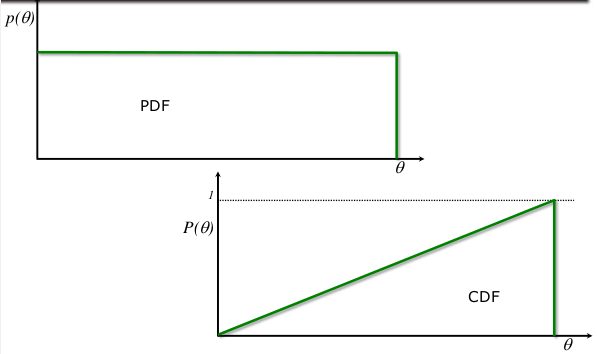
\includegraphics[height=2.75in,clip]{cont-pdf-cdf}
	\end{center}
  	\end{figure}

\end{frame}


%%%%%%%%%%%%%%%%%%%%%%%%%%%%%%%%%%%%%%%%%%%%%%%%%%%%%%
%%%%%%%%%%%%%%%%%%%%%%%%%%%%%%%%%%%%%%%%%%%%%%%%%%%%%%
\begin{frame}{Random Sampling Basics}

  	\begin{figure}
  	\begin{center}
  		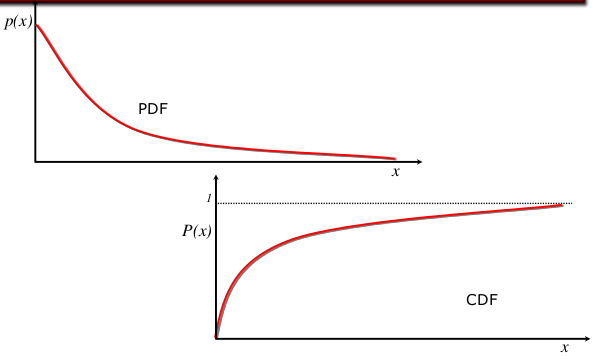
\includegraphics[height=2.75in,clip]{cont-pdf-cdf-2}
	\end{center}
  	\end{figure}

\end{frame}

%%%%%%%%%%%%%%%%%%%%%%%%%%%%%%%%%%%%%%%%%%%%%%%%%%%%%%
%%%%%%%%%%%%%%%%%%%%%%%%%%%%%%%%%%%%%%%%%%%%%%%%%%%%%%
\begin{frame}{Random Sampling Basics}

  	\begin{figure}
  	\begin{center}
  		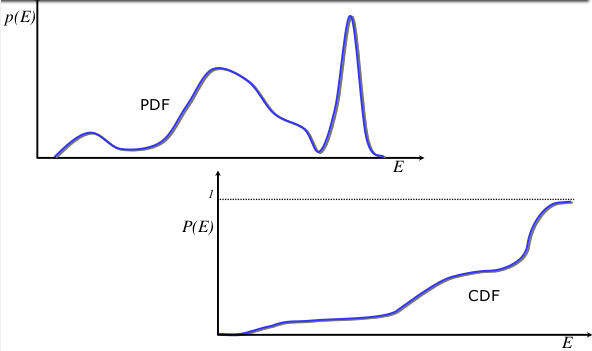
\includegraphics[height=2.75in,clip]{cont-pdf-cdf-3}
	\end{center}
  	\end{figure}

\end{frame}

%%%%%%%%%%%%%%%%%%%%%%%%%%%%%%%%%%%%%%%%%%%%%%%%%%%%%%
%%%%%%%%%%%%%%%%%%%%%%%%%%%%%%%%%%%%%%%%%%%%%%%%%%%%%%
\begin{frame}{Random Sampling Basics}

  	\begin{figure}
  	\begin{center}
  		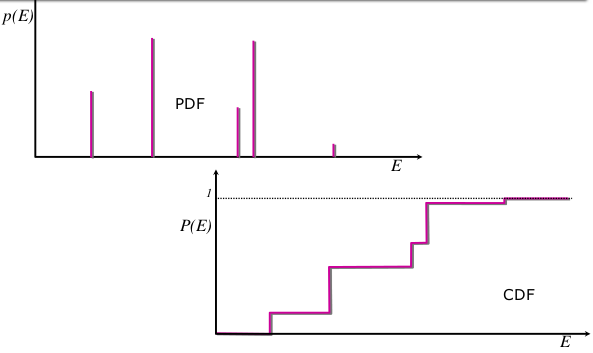
\includegraphics[height=2.75in,clip]{disc-pdf-cdf}
	\end{center}
  	\end{figure}

\end{frame}


%%%%%%%%%%%%%%%%%%%%%%%%%%%%%%%%%%%%%%%%%%%%%%%%%%%%%%
%%%%%%%%%%%%%%%%%%%%%%%%%%%%%%%%%%%%%%%%%%%%%%%%%%%%%%
\begin{frame}{Why Random Sampling}

Various physical phenomena can be
represented by probabilistic distributions

\begin{itemize}
    \item The known probability distribution
represents the \textit{collective} behavior
\vspace*{1em}
    \item We need to know the behavior at \textit{each}
single event
\vspace*{1em}
    \item We need to \underline{recreate} the collective behavior after \underline{many} events
\end{itemize}

\end{frame}


%%%%%%%%%%%%%%%%%%%%%%%%%%%%%%%%%%%%%%%%%%%%%%%%%%%%%%
%%%%%%%%%%%%%%%%%%%%%%%%%%%%%%%%%%%%%%%%%%%%%%%%%%%%%%
\begin{frame}{Random Sampling Purpose}

Use a random process to select a single
value with the following requirements

\begin{itemize}
    \item Each sample should be independent from
other samples
\vspace*{1em}
    \item The PDF formed from a large number of
samples should converge to the initial PDF
\vspace*{1em}
    \item Recover the full resolution of the initial PDF
\end{itemize}

\end{frame}


%%%%%%%%%%%%%%%%%%%%%%%%%%%%%%%%%%%%%%%%%%%%%%%%%%%%%%
%%%%%%%%%%%%%%%%%%%%%%%%%%%%%%%%%%%%%%%%%%%%%%%%%%%%%%
\begin{frame}{Sampling Techniques}

Random sampling uses \underline{uniformly distributed
random variables} to \alert{choose a value for a
variable} according to its probability density
function

    \begin{itemize}
    \item \textit{Basic} sampling techniques
      \begin{itemize}
      \item Direct discrete sampling
      \item Continuous discrete sampling
      \item Rejection sampling
      \end{itemize}
    \pause
    \vspace*{.5em}
    \item \textit{Advanced }sampling techniques
      \begin{itemize}
      \item Histogram
      \item Piecewise linear
      \item Alias sampling
      \item Advanced continuous PDFs
      \end{itemize}
    \end{itemize}

\end{frame}


%%%%%%%%%%%%%%%%%%%%%%%%%%%%%%%%%%%%%%%%%%%%%%%%%%%%%%
%%%%%%%%%%%%%%%%%%%%%%%%%%%%%%%%%%%%%%%%%%%%%%%%%%%%%%
\begin{frame}{Uniformly-Distributed Random Variable}

    \begin{itemize}
    \item Standard notation
      \begin{itemize}
      \item Single random variable: $\xi$
      \item Pair of random variables: $(\xi, \eta)$
      \end{itemize}
    \vspace*{.5em}
    \item PDF for random variables:
    \end{itemize}

\begin{columns}
  \begin{column}{0.5\textwidth}
    %
    \begin{align*}
    p(\xi) = \begin{cases} 
     1 & 0 \leq \xi < 1 \\ 
     0 & \text{ otherwise} 
     \end{cases}
    \end{align*}
  \end{column}
  \begin{column}{0.5\textwidth}
  	\begin{figure}
  	\begin{center}
  		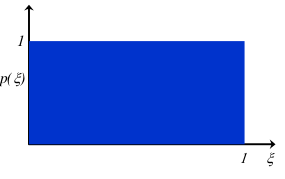
\includegraphics[height=1.5in,clip]{unif-dist-var}
	\end{center}
  	\end{figure}
  \end{column}
\end{columns}

\end{frame}


%%%%%%%%%%%%%%%%%%%%%%%%%%%%%%%%%%%%%%%%%%%%%%%%%%%%%%
%%%%%%%%%%%%%%%%%%%%%%%%%%%%%%%%%%%%%%%%%%%%%%%%%%%%%%
\begin{frame}{Direct Discrete Sampling}

Sampling Procedure

    \begin{itemize}
    \item Generate $\xi$
    \item Determine $k$ such that $P_{k-1} \leq \xi \leq P_k$
    \item Return $x = x_k$
    \end{itemize}

  	\begin{figure}
  	\begin{center}
  		\includegraphics<1>[height=1.5in,clip]{disc-pdf}
  		\includegraphics<2>[height=1.5in,clip]{disc-pdf-samp}
	\end{center}
  	\end{figure}

\end{frame}


%%%%%%%%%%%%%%%%%%%%%%%%%%%%%%%%%%%%%%%%%%%%%%%%%%%%%%
%%%%%%%%%%%%%%%%%%%%%%%%%%%%%%%%%%%%%%%%%%%%%%%%%%%%%%
\begin{frame}{Direct Discrete Sampling}

\vspace*{1 em}
Consider the CDF

  	\begin{figure}
  	\begin{center}
  		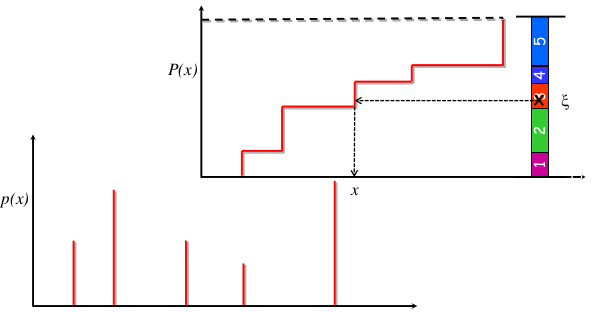
\includegraphics[height=2.5in,clip]{disc-cdf}
	\end{center}
  	\end{figure}

\end{frame}



\end{document}
